\chapter{Simulator and data capture}\label{app5}

This appendix presents the modelling techniques applied to the simulator and discusses the processes used to analyse the datasets produced by the simulations.

\section{Swarm simulator object model}\label{sim:Simulator3}
Figure~\ref{sim:objectModel} shows the object model underlying the simulator. The \texttt{\textbf{World}} class models the Euclidean plane for the simulations. The \texttt{\textbf{World}} class is a container object for other classes including lists of swarms, destinations, and obstacles that make up the environment to be modelled. The \texttt{\textbf{Swarm}} class implements a list which contains several \texttt{\textbf{Participants}} (agents) that constitute a swarm. The \texttt{\textbf{Participant}} class models the swarm agents and inherits the \texttt{\textbf{Bot}} class which provides the positioning coordinates for the agents. The \texttt{\textbf{Destination}} and \texttt{\textbf{Obstacle}} classes inherit their coordinates from the \texttt{\textbf{Bot}} class. The \texttt{\textbf{Swarm}} class implements a generic physics model for the coordination of the agents. The \texttt{\textbf{BoidSwarm}} class inherits the \texttt{\textbf{Swarm}} class and implements the algorithm for the boid model which includes the physics modelling. The \texttt{\textbf{Logger}} class implements a data logging mechanism and is used to capture the simulation data from within the \texttt{\textbf{World}} class via the \texttt{\textbf{Global}} class which is an implementation of a singleton containing the environmental constraints.

\begin{figure}[H]
\begin{center}
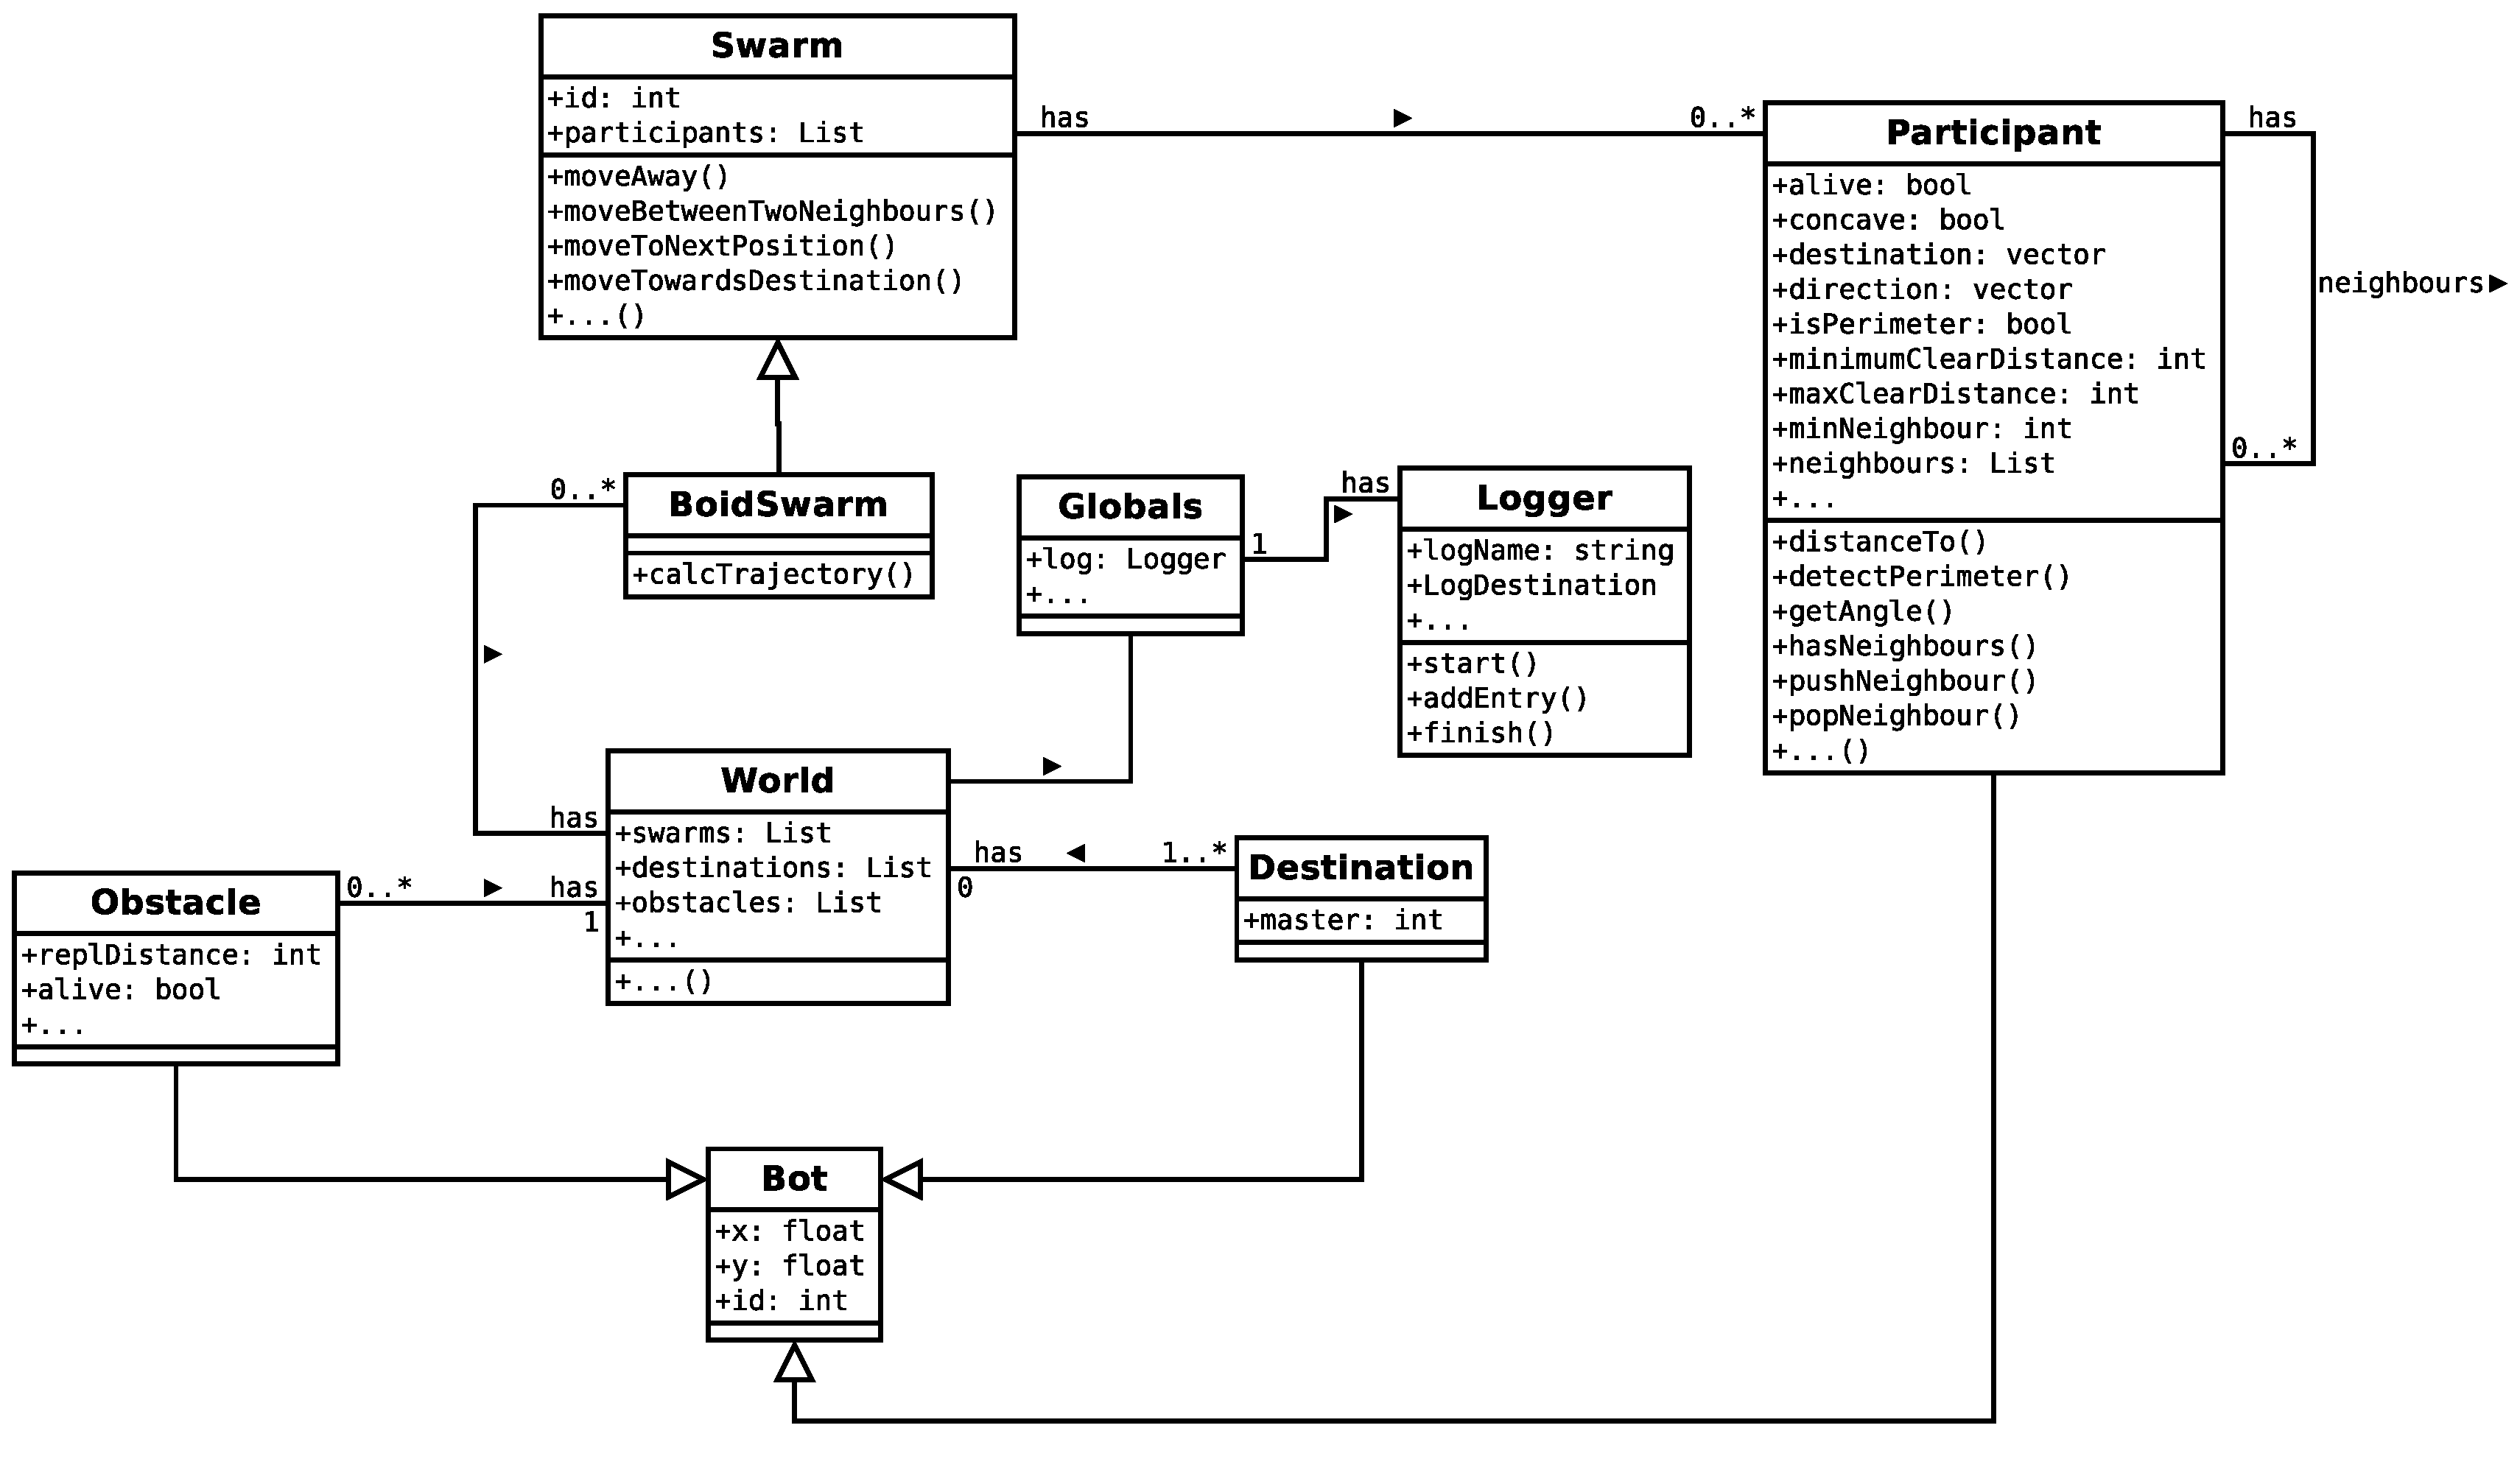
\includegraphics[width=13cm]{CHAPTER-3/figures/classes_World}
\end{center}
\caption[Simulator object model]{Simulator object model}\label{sim:objectModel}
\end{figure}

The object modelling shown in Figure~\ref{sim:objectModel} is implemented in Python using packages.

The complete PySwarmWorld application is available at \url{https://drive.google.com/file/d/0B0DIRBx-V-eYVnNvVEkzUkRuZVk/view?usp=sharing}.

\section{Simulator data capture}

When data logging is activated the simulator generates an SQL log file using the \textbf{Logger} Class. As the simulation runs the system, at each time interval~($t$) calculates all of the agents movements and the magnitudes that affect each agent pair generate. This data is then appended to the SQL log file as a transaction~(Listing~\ref{code:SQL2}), shown as (3a) in~figure~\ref{sim:SimulatorOverview} on page~\pageref{sim:SimulatorOverview}, using the~\texttt{\textbf{addEntry()}} method of the~\texttt{\textbf{Logger}} class. This method generates two SQL insertions that are added for each transaction. 

The agent data is added to the log file and it consists of the positional information of the agent along with the destination and directional bias the agent has affecting it. There are also the statistics of the minimum and maximum distances of its neighbours and a boolean flag identifying if the agent is on a perimeter. If an agent is on a perimeter it will be affected by a destination vector. The second set of entries are the neighbour records which include the physics data the neighbour has affecting it through that relationship. 

When a simulation is finished the SQL log is closed. 

\section{Data capture implementation}
The code in~listing~\ref{code:SQL2} shows how the log entries for a simulation run are captured. Line~\ref{line:participantSQL} shows the agent details embedded in an SQL insert statement. This statement is then appended to the log file using the \texttt{\textbf{addEntry()}} method. The code then iteration over the agents~\texttt{\textbf{bot.neighbours}} list (Line~\ref{line:neighbourList}). On line~\ref{line:neighbourSQL} the neighbour entries are added to the log file using the \texttt{\textbf{addEntry()}} method.

\lstset{language=Python,
basicstyle=\tiny,
numbers=left, 
numberstyle=\tiny,
captionpos=b,
keepspaces=true,
showspaces=false, 
showstringspaces=false,
showtabs=false,
frame=single,
breaklines=true,
caption=Simulator data capture,
escapechar=|
} % Set your language (you can change the language for each code-block optionally)
\begin{lstlisting}[label={code:SQL2}]  % Start your code-block

|\label{line:participantSQL}|status.log.addEntry("INSERT INTO PARTICIPANT VALUES (%s,%s,%s,%s,%s,%s,%s,%s,%s,%s,%s,%s,%s,%s,%s,%s);\n" % (status.logCount,timeStamp,bot.id,bot.x,-bot.y,bot.direction.x,bot.direction.y,bot.destination.x,bot.destination.y,bot.alive, bot.distanceTravelled,bot.scanCounter,bot.minNeighbour,bot.maxNeighbour,bot.isPerimeter,bot.scanning))
|\label{line:neighbourList}|for neighbour in bot.neighbours:
  distanceToNeighbour = Vector2.from_points((bot.x, bot.y),(neighbour.x, neighbour.y))
  repulsion = (((bot.minimumClearDistance - distanceToNeighbour.get_length()) /distanceToNeighbour.get_length()) * bot.minimumClearDistance) * status.physicsMoveAway
  cohesion = distanceToNeighbour.get_length() * status.physicsFlyTowardsCentre
  resultant = cohesion - repulsion
  |\label{line:neighbourSQL}|status.log.addEntry("INSERT INTO NEIGHBOUR VALUES (%s,%s,%s,%s,%s,%s,%s);\n" % (status.logCount,bot.id,neighbour.id,distanceToNeighbour.get_length(),resultant,cohesion,repulsion))
\end{lstlisting}

\section{Data capture tables}
The tables created from the initial log file are the starting point of the analysis process. 

\subsection{\texttt{\textbf{PARTICIPANT}} table (Agents)}
The \texttt{\textbf{PARTICIPANT}} table~\ref{code:Participant} is a snapshot of all the agents in the swarm at each time interval. The data that is logged includes the position (\texttt{\textbf{x}},\texttt{\textbf{y}}) of each agent along with the direction of the agent (\texttt{\textbf{directionX}}, \texttt{\textbf{directionY}}). The table also includes the field effect values for repulsion~(\texttt{\textbf{minNeighbour}}) and cohesion~(\texttt{\textbf{maxNeighbour}}). The table is used for several aggregations and also to plot the path of individual agents within a simulation.

\subsection{\texttt{\textbf{NEIGHBOUR}} table} 
The \texttt{\textbf{NEIGHBOUR}} table~\ref{code:Neighbour} is a snapshot of all the agents that are `visible' to an agent. This table is directly related to the \texttt{\textbf{PARTICIPANT}} table via the \texttt{\textbf{LogCount}} and \texttt{\textbf{id}} fields as a one to many relationship. This table also contains the calculated magnitudes for the repulsion and cohesion of each neighbour to its parent. The table also includes the calculated distance the neighbour is away from the parent agent. 

\section{Simulator data aggregation}
Following the simulation the SQL log file is imported into an `analysis' database. This is shown as (3b) in~figure~\ref{sim:SimulatorOverview}~on~page~\pageref{sim:SimulatorOverview}. Once the base data is loaded into the database the aggregation of the data can be executed.

\subsection{Data aggregation views}
The data aggregation is shown as stage (4) in~figure~\ref{sim:SimulatorOverview} on page~\pageref{sim:SimulatorOverview}. The aggregated views of the data provide a deeper level of information that is required for the analyse of the internal activity of the swarm.

There are several steps in the aggregation of the base data. Each step builds up a set of persistent views. The views expose the `dynamics' of the swarm at each time interval. The views are persistent to improve the query time of the simulation analysis. This technique is used as the data, once captured, is static. The data model for the swarm dynamics database is shown in~figure~\ref{app3:schema} on page~\pageref{app3:schema}. The following sections give a breakdown of the aggregation views and their purpose.

\subsubsection{\texttt{\textbf{LOGS}} view}
The \texttt{\textbf{LOG}} view~(Listing~\ref{code:LOGS}) is an aggregation of the time intervals in the simulation. It includes a counter which is a sequence number for each time increment in the system and a timestamp in seconds of the current simulation runtime.

\subsubsection{\texttt{\textbf{SWARM}} view}
The \texttt{\textbf{SWARM}} view~(Listing~\ref{code:SWARM}) allows the centroid of the swarm to be tracked. This allows the position of a swarm to be monitored based on its centre of mass. The view takes into account agents that have been removed from the swarm by only selecting `live' agents from the base data. The view also provides a count of the number of live agents that are currently in the swarm.

\subsubsection{\texttt{\textbf{PERIMETER}} view}
The \texttt{\textbf{PERIMETER}} view~(Listing~\ref{code:PERIMETER}) provides a list of the agent identifiers (\texttt{\textbf{id}}) that have their perimeter status flag~(\texttt{\textbf{isPerimeter}}) set to \texttt{\textbf{TRUE}} in a specific time slice~(\texttt{\textbf{logCount}}).

\subsubsection{\texttt{\textbf{FULLPERIMETER}} view}
The \texttt{\textbf{FULLPERIMETER}} view~(Listing~\ref{code:FULLPERIMETER}) aggregates the \texttt{\textbf{PERIMETER}} view to provide a total~(\texttt{\textbf{SIZE}}) of how many agents have their perimeter flag~(\texttt{\textbf{isPerimeter}}) set. These agents may be influencing a swarms direction. This allows changes in the perimeter size to me monitored as a simulation progresses.

\subsubsection{\texttt{\textbf{SWARMSIZE}} view}
The \texttt{\textbf{SWARMSIZE}} view~(Listing~\ref{code:SWARMSIZE}) provides a running total of the total number of agents that are active in a swarm. This allows the detection of agent loss in a simulation.

\subsubsection{\texttt{\textbf{FULLNEIGHBOUR}} view}
The \texttt{\textbf{FULLNEIGHBOUR}} view~(Listing~\ref{code:FULLNEIGHBOUR}) provides a running total, for each time slice, of the number of neighbours each agent has. This allows the expansion phase of a swarm to be monitored. This view can also be used to identify if the cohesion and repulsion weightings and distances allow the swarm to create hexagonal lattices.

\subsubsection{\texttt{\textbf{NEIGHBOURDISTANCE}} view}
The \texttt{\textbf{NEIGHBOURDISTANCE}} view~(Listing~\ref{code:NEIGHBOURDISTANCE}) provides access to the distances between each agent in the swarm and its neighbours. This allows the analysis of the swarms structure based on inter-agent distances. The inter-agent distances are the swarm attribute identified by Navarro and Mat{\'\i}a in their swarm metrics paper~\cite{NIM:09}. The view also provides access to the magnitudes of the cohesion, repulsion and resultant magnitude for each agent-neighbour relationship. These three attributes allow a more detailed view of the state of the swarm to be identified. These attributes highlight a swarms structural `performance'. This view also includes the maximum and minimum magnitudes and provides a `picture' of the swarm's distribution which can be realised graphically.

\subsubsection{\texttt{\textbf{SWARMTRAVELLED}} view}
The \texttt{\textbf{SWARMTRAVELLED}} view~(Listing~\ref{code:SWARMTRAVELLED}) provides the total distance travelled by all the agents in the swarm. This information can be used to compare the distance each agent has travelled to the distance the centroid of the swarm has travelled. This creates a measure to identify the efficiency of the perimeter influence on a swarm's directional movement.

\subsubsection{\texttt{\textbf{DISTANCEGPS}} view}
The \texttt{\textbf{DISTANCEGPS}} view~(Listing~\ref{code:DISTANCEGPS}) provides the total distance travelled by agents that have GPS sensors enabled and are coordinating the swarm. This information can be used to identify the degree of GPS influence on the movement of a swarm. 

\subsubsection{\texttt{\textbf{SWARMPROFILE}} view}
The \texttt{\textbf{SWARMPROFILE}} view~(Listing~\ref{code:SWARMPROFILE}) identifies the centroid of the swarm at each time interval. It also provides general information about how large the swarm is and the distance travelled by the agents.

A copy of all of the experimental data extracts is available at: \url{https://drive.google.com/file/d/0B0DIRBx-V-eYTVNQeFVEUFlOMEk/view?usp=sharing}.

\section{Data graphing tools}\label{sim:GraphingTools}
The resultant views allow the visualisation of the swarm activity. The data realisation tool used in this thesis is \texttt{\textbf{matplotlib}}~\cite{JH:16}. This is a python-based graphing environment which provides facilities similar to \texttt{\textbf{MatLab}}~\cite{MATLAB:94}. 

The aggregated data is extracted from the MySQL~\cite{OC:16} database using the \texttt{\textbf{cymsql}} MySQL connector~\cite{PSF:15}~shown as (5) in~figure~\ref{sim:SimulatorOverview}~on~page~\pageref{sim:SimulatorOverview}. The data when extracted is applied to a specific plot type. These plots are then rendered to visualise the characteristics of the swarm, this is shown as (6) in~(figure~\ref{sim:SimulatorOverview}).

The sample code~(Listing~\ref{code:Graph1}) is for a simple path plot for a swarm. Line~\ref{line:fetchRecords} shows the iteration over the records extracted from the database using the \texttt{\textbf{cymysql}} connector (Line~\ref{line:cymysqlConn}). The data is then pushed into two lists ($x[~]$,$y[~]$), shown in~(Lines \ref{line:arrayx} and \ref{line:arrayy}). Line~\ref{line:plotType} shows the selection of the plot type (\texttt{\textbf{plot}}) and line~\ref{line:plotShow} generates the graph~(\texttt{\textbf{show}}). An example of the graph this generates, a swarm's centroid path, is shown in~figure~\ref{sim:sampleGraph} on page~\pageref{sim:sampleGraph}. 

\lstset{language=Python,
basicstyle=\tiny,
numbers=left, 
numberstyle=\tiny,
captionpos=b,
frame=single,
breaklines=true,
caption=Sample \texttt{\textbf{matplotlib}} script,
escapechar=|
} % Set your language (you can change the language for each code-block optionally)
\begin{lstlisting}[label={code:Graph1}]  % Start your code-block

#!/usr/bin/python3
import cymysql
import matplotlib.pyplot as plt

x = []
y = []

|\label{line:cymysqlConn}|conn = cymysql.connect(host='127.0.0.1', user='phd', passwd='*********', db='ST-TEST3-20S', charset='utf8')
cur = conn.cursor()
cur.execute('SELECT * FROM SWARM')
|\label{line:fetchRecords}|for r in cur.fetchall():
|\label{line:arrayx}|    x.append(r[1])
|\label{line:arrayy}|    y.append(-r[2])

|\label{line:plotType}|p = plt.plot(x,y, label="Baseline",color="k", linewidth=1)
plt.title('Swarm Path Propagation (200)',fontsize=30)
plt.ylabel('y',fontsize=30)
plt.xlabel('x',fontsize=30)
plt.legend(fontsize=30)

|\label{line:plotShow}|plt.show()
\end{lstlisting}

\begin{figure}[H]
\begin{center}
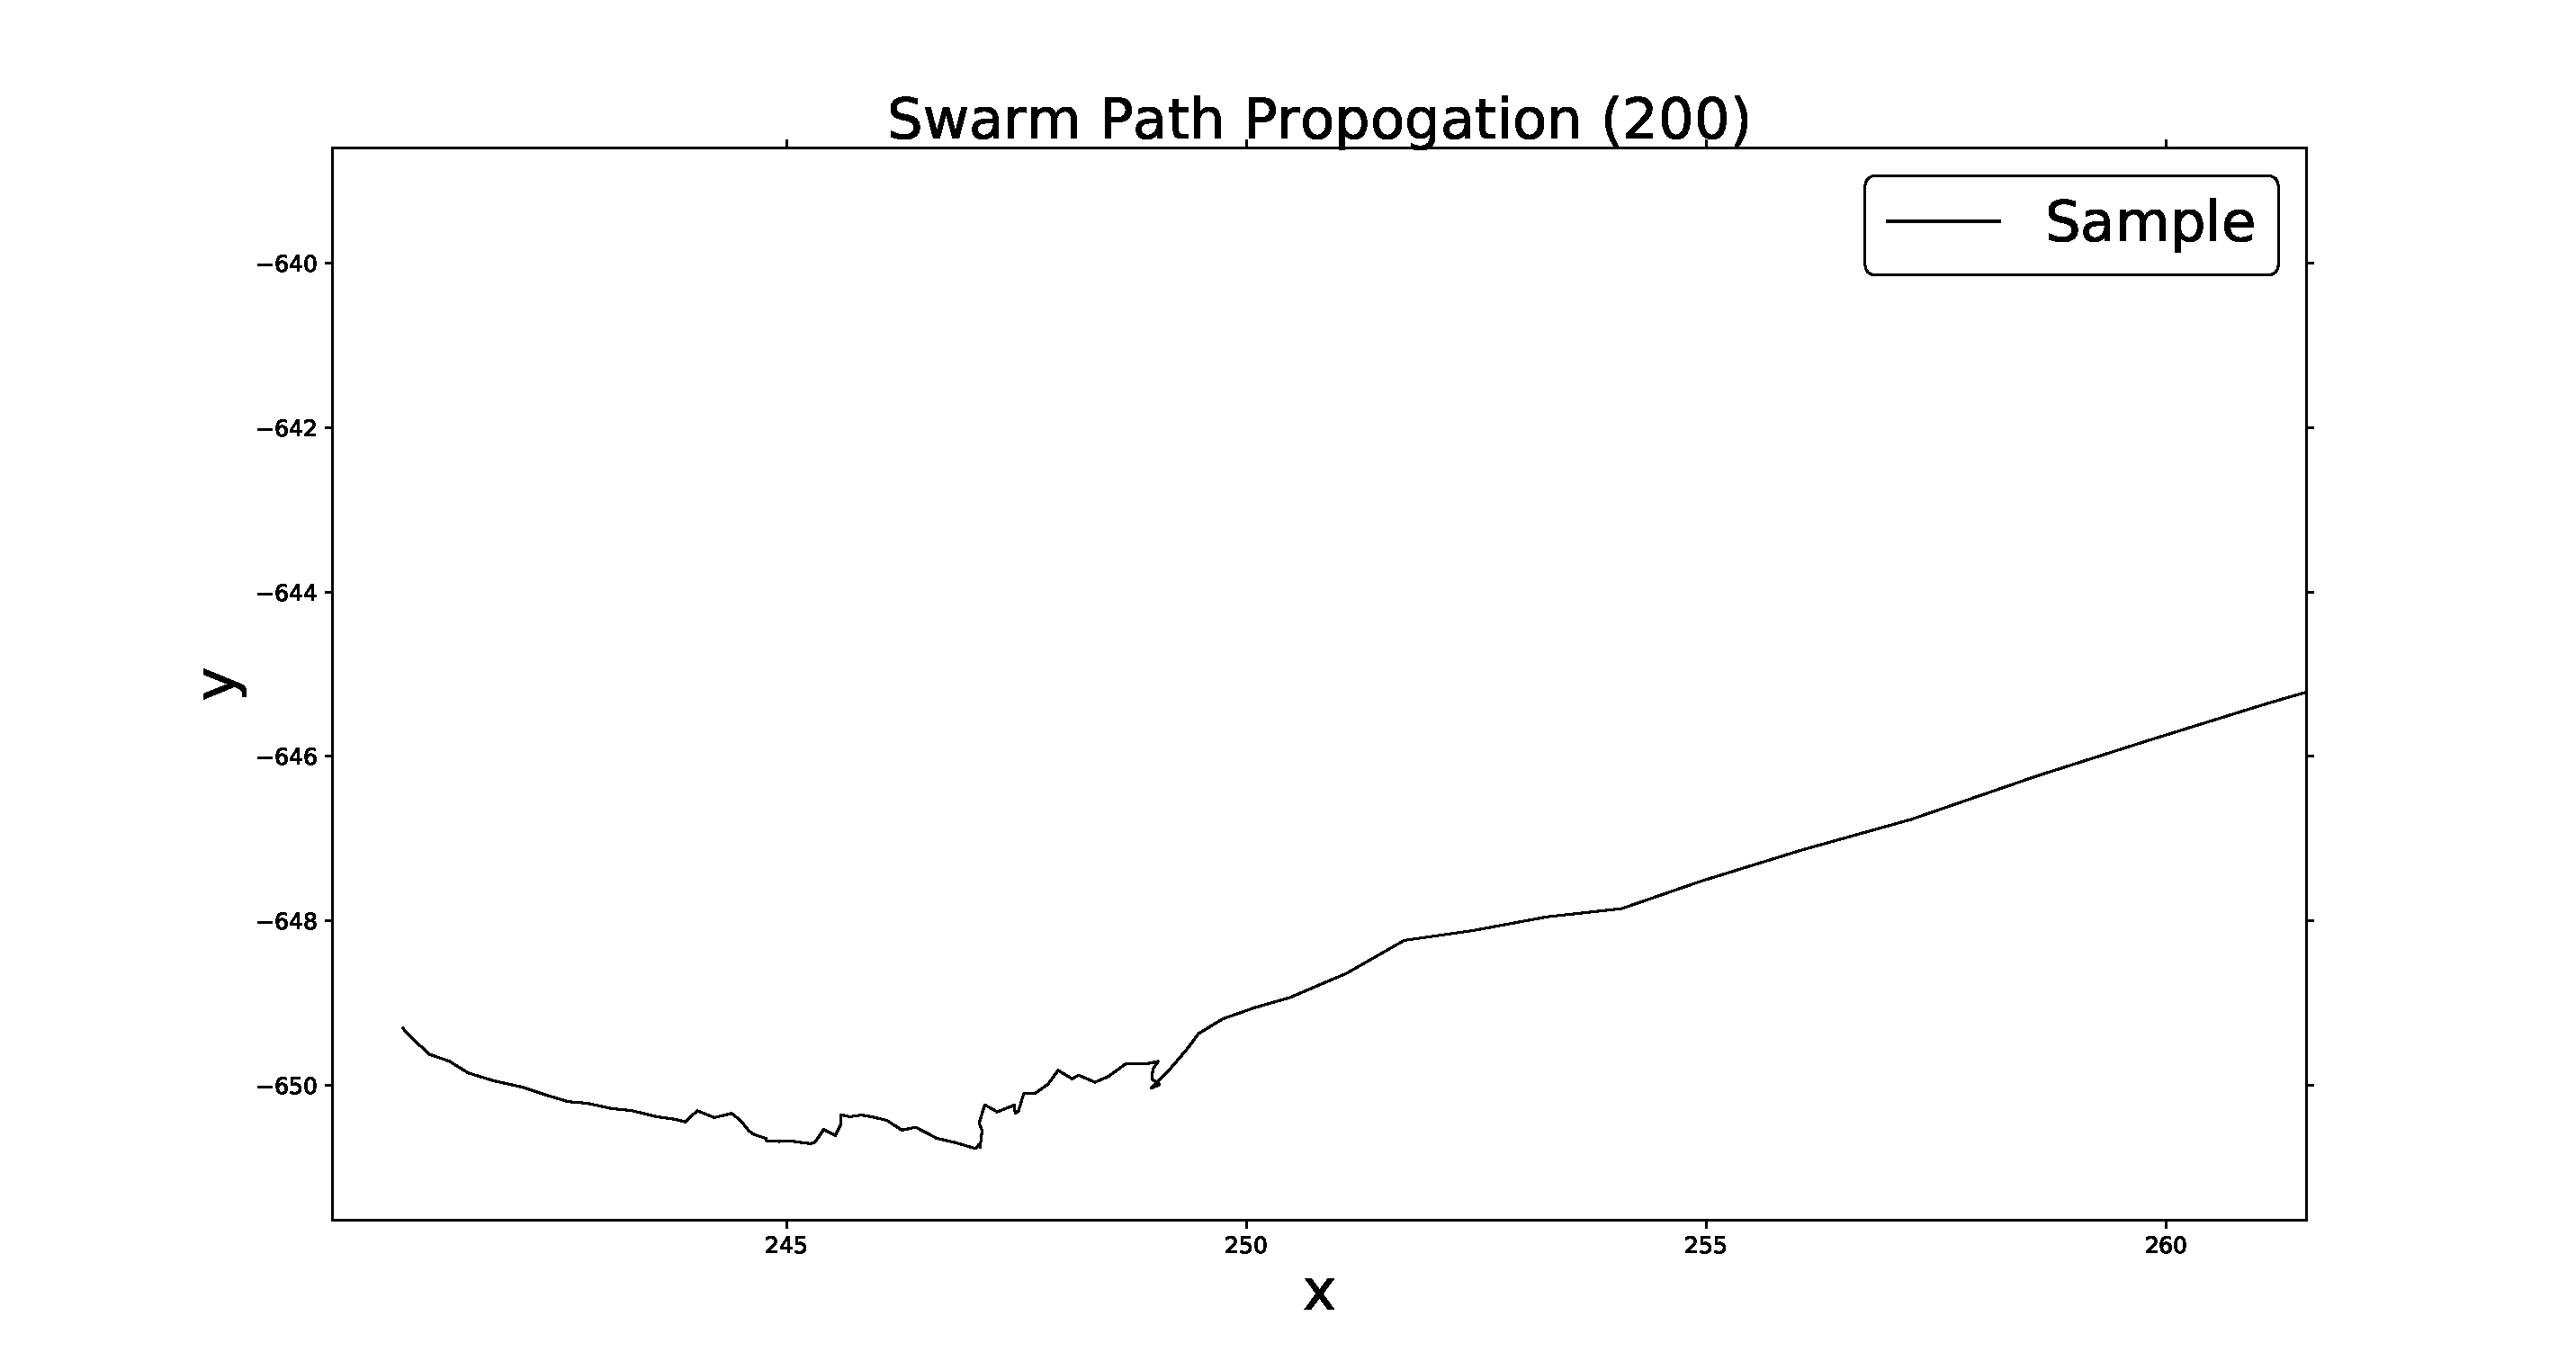
\includegraphics[width=15cm]{CHAPTER-3/figures/SampleGraph}
\end{center}
\caption[Sample graph]{Sample \texttt{\textbf{matplotlib}} graph}\label{sim:sampleGraph}
\end{figure}

A copy of all of the graphing scripts is available at: \url{https://drive.google.com/file/d/0B0DIRBx-V-eYVVg1T1JXREx2eGM/view?usp=sharing}.
